
\documentclass[conference]{IEEEtran}
% Add the compsoc option for Computer Society conferences.
%
% If IEEEtran.cls has not been installed into the LaTeX system files,
% manually specify the path to it like:
% \documentclass[conference]{../sty/IEEEtran}





% Some very useful LaTeX packages include:
% (uncomment the ones you want to load)


% *** MISC UTILITY PACKAGES ***
%
%\usepackage{ifpdf}
% Heiko Oberdiek's ifpdf.sty is very useful if you need conditional
% compilation based on whether the output is pdf or dvi.
% usage:
% \ifpdf
%   % pdf code
% \else
%   % dvi code
% \fi
% The latest version of ifpdf.sty can be obtained from:
% http://www.ctan.org/tex-archive/macros/latex/contrib/oberdiek/
% Also, note that IEEEtran.cls V1.7 and later provides a builtin
% \ifCLASSINFOpdf conditional that works the same way.
% When switching from latex to pdflatex and vice-versa, the compiler may
% have to be run twice to clear warning/error messages.







%
\ifCLASSINFOpdf
  % \usepackage[pdftex]{graphicx}
  % declare the path(s) where your graphic files are
  % \graphicspath{{../pdf/}{../jpeg/}}
  % and their extensions so you won't have to specify these with
  % every instance of \includegraphics
  % \DeclareGraphicsExtensions{.pdf,.jpeg,.png}
\else
  % or other class option (dvipsone, dvipdf, if not using dvips). graphicx
  % will default to the driver specified in the system graphics.cfg if no
  % driver is specified.
  % \usepackage[dvips]{graphicx}
  % declare the path(s) where your graphic files are
  % \graphicspath{{../eps/}}
  % and their extensions so you won't have to specify these with
  % every instance of \includegraphics
  % \DeclareGraphicsExtensions{.eps}
\fi


% correct bad hyphenation here
\hyphenation{op-tical net-works semi-conduc-tor}
\usepackage[utf8]{inputenc}
\usepackage{graphicx}
\usepackage{capt-of}

\begin{document}
%
% paper title
% can use linebreaks \\ within to get better formatting as desired
\title{Human and Autonomous Robot Competition}


% author names and affiliations
% use a multiple column layout for up to three different
% affiliations
\author{
\IEEEauthorblockN{João Henriques, Joaquim Oliveira}
\IEEEauthorblockA{Engenharia Informatica e computação\\
Faculdade de Engenharia\\
Univercidade do Porto\\
Porto, Portugal\\
Email: joaoh88@gmail.com, jjsfoliveira@gmail.com}
}





% make the title area
\maketitle


\begin{abstract}
Currently the Man vs Machine competition is the center of many scientific researches. In this scientific article, we will describe an implementation of a competition between autonomous robots and robots controlled by humans. 

Robots, sensor, algorithm, competition, simulator (key words)

\end{abstract}

\IEEEpeerreviewmaketitle



\section{Introdução}
Nos dias de hoje, na sociedade moderna, os robôs e a tecnologia têm vindo a assumir um papel cada vez mais importante nas nossas vidas. A ideia de que um robô pode substituir um ou vários humanos nas activades mais banais e repetitivas do quotidiano tem sido o principal motivo de todos os desenvolvimentos cientificos e tecnológicos que temos tido oportunidade de assistir nestes últimos anos. Seja desde o aparecimento das linhas de produção ou de montagem numa mega fábrica, onde os humanos passaram a ocupar o simples papel de monitorização de toda a maquinaria envolvida nesse processo, até o aparecimento dos agora muito populares robôs de cozinha, é nos quase impossível imaginar uma sociedade em que não existam todos estes gadgets que proporcionam o comodismo que já todos damos como garantido.

Serão de facto os robôs realmente capazes de concluir as tarefas repetitivas do dia-a-dia que nós não queremos fazer? E serão estes melhores do que nós?

A resposta à maioria destas e outras possíveis questões que poderiam ser colocadas, podem à partida parecer muito simples, mas muitas vezes esquecemo-nos da complexidade envolvida e necessária para serem atingidos os mais simples dos objectivos \cite{IEEEhowto:h_vs_r}.

Um desafio que pode excitar a sociedade é o “duelo” Humanos \textit{vs.} Máquinas. Neste artigo vamos apresentar uma competição criada por nós utilizando um ambiente virtual, o \textit{CiberRato} \cite{IEEEhowto:rato_s}, onde vários robôs controlados por humanos ou com autonomia própria competem entre si, vencendo quem chegar ao objectivo primeiro. Embora esta não seja uma forma de podermos demonstrar se somos melhores ou não que máquinas criadas por nós, é uma boa forma de visualizar como é difícil criar um robô que faça exactamente aquilo que pretendemos e de forma exacta.

\section{Problema}

O objectivo desta aplicação passa por através do simulador CiberRato criar uma competição entre Humanos e Máquinas, onde é possível demonstrar a dificuldade ou facilidade de criar um robô que seja realmente melhor que um humano nas tarefas mais banais. Para isso é necessário desenvolver dois tipos de robôs, uns controlados por humanos (joystick) e outros controlados com autonomia própria.

De forma a tornar o desafio mais interessante decidimos “esconder” o ambiente gráfico disponível pelo \textit{CiberMouse} e desenvolver um novo para que numa fase inicial não tenhamos qualquer informação sobre o mapa e á medida que o vamos explorando vamos o conhecendo através da informação disponível pelos vários sensores.

Quanto ao robô com autonomia própria pretende-se que através dos seus sensores seja capaz de tomar as melhores decisões, desviando-se dos diferentes obstáculos e dirigindo-se para o alvo. 

\section{CiberMouse}

O \textit{CiberMouse} ou \textit{CiberRato} é uma competição de robôs que ocorre em ambiente simulado. O ambiente é constituído por uma arena virtual, composta por obstáculos e por duas áreas distintas, uma representando o local de partida (onde os robôs virtuais começam e onde têm de se dirigir no final) e outra representando o alvo (que têm de o ir buscar) \cite{IEEEhowto:ciberrato}.

Os robôs têm todos o mesmo tamanho e forma (redonda) sendo equipados por sensores, atuadores e botões de comando (Fig. 1). O principal objectivo é começando todos na mesma posição alcançar o alvo e regressar á posição inicial. Pelo percurso estes têm de ter a capacidade de se desviarem dos diferentes obstáculos, podendos estes serem estáticos ou mesmo outros robôs a participar na competição.

Todos os robôs ficam bloqueados dentro da área do alvo à medida que vão chegando, sendo apenas no momento da chegada do último que voltam a ser desbloqueados e podem regressar à origem.

Cada robô possui varios tipos de sensores. Sendo estes: quatro sensores de obstáculos (ajudam a determina a posição dos obstáculos relativamente ao robô), um sensor de alvo (indica o ângulo do robô relativamente ao alvo), uma bússola (indica a rotação do robo), um sensor de colisão (indica se o robô está em contacto com algum obstaculo), um sensor de terreno (determina se o robô está completamente dentro da área de alvo ou da área de início) e um GPS (indica a posição do robô). A finalidade destes é recolher e transmitir o estado actual do ambiente virtual que rodeia o robô, de forma a conseguir desviar-se dos obstáculos e alcançar o objectivo.

A utilização do \textit{CiberRato} virtual neste projecto tem como objectivo tornar a competição o mais realista possível pois possui excelentes recursos que permitem uma fácil implementação do problema descrito.


\begin{figure}
\centering
 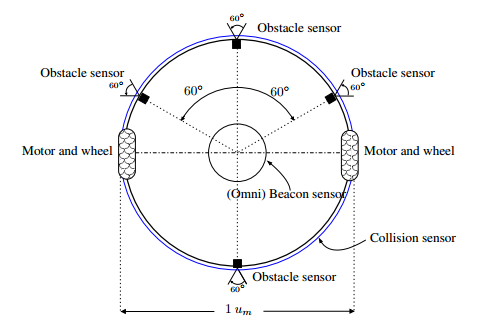
\includegraphics[width=0.4\textwidth]{image/ciberMouse.png}
\caption{Corpo de um robô virtual}
\label{fig:patches}
\end{figure}

\section{Solução implementada}
Como já foi indicado anteriormente foi implementado dois tipos diferentes de robôs: um autónomo e outro controlado por um humano através de um joystick.

\subsection{Robô autónomo}
A solução implementada tem por base dois estados distintos: o “Run” e o “Return”. No primeiro caso o agente percorre o ambiente á procura do alvo, tendo de se desviar dos diferentes obstáculos ou de outros robôs, no segundo caso o robô depois de ter encontrado o alvo, procura a área de início. 

Em ambos é necessário determinar, em cada instante, a próxima acção (deslocar-se segundo o eixo frontal, rodar, desviar-se de algum obstáculo ou dirigir-se para o local do alvo). Para isso a informação obtida através dos sensores é de grande importância. Utilizando esta informação implementamos um algoritmo de forma a determinar a potência a fornecer a cada motor. Os principais momentos de decisão são:

\begin{enumerate}
\item Através do sensor de colisão e do sensor de obstáculos frontal determina se o robô está a ser bloqueado por algum tipo de obstáculo. Se sim o robô roda mudando assim o sentido do seu movimento;
\item Se for possível visualizar o alvo (sensor de alvo) o robô muda de sentido de forma a se dirigir para este;
\item Se existir algum obstáculo próximo de alguma lateral e da parte frontal o robô roda, mudando de direcção de forma a evitar o contacto;
\item Se existir algum obstáculo próximo da lateral o robô muda de sentido de forma a não colidir com o obstáculo. A mudança de direcção é inversamente proporcional á distância.
\end{enumerate}

\subsection{Robô controlado por humanos}
De forma a criar um segundo ambiente gráfico dividimos a nossa solução em duas parte. Na primeira foi desenvolvido o robô escrito em linguagem C, baseado no \texit{sample} que é distribuído com o próprio simulador do \textit{CiberRato}, sendo aqui que o joystick é utilizado para comunicar com os motores do robô de forma a controlar o seu movimento e onde são recolhidos os valores dos sensores disponíveis e enviados através de um socket para a segunda parte desta aplicação, o visualizador.

\begin{figure}
\centering
 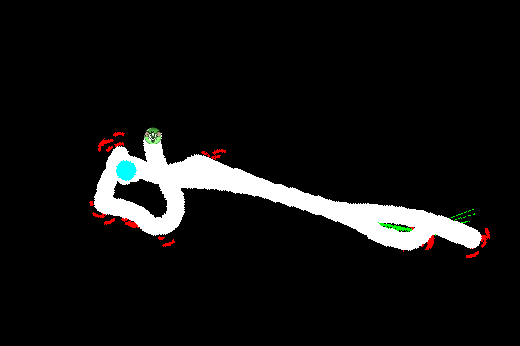
\includegraphics[width=0.4\textwidth]{image/untitled2.png}
\caption{Janela do Viewer}
\label{fig:screen}
\end{figure}

O visualizador foi desenvolvida em java e é responsável por representar gráficamente os dados dos sensores recolhidos, sendo estes trabalhados de forma a representar o conhecimento que foi possível obter deste o início da partida. É de referir que no início é apenas apresentado ao utilizador um ecrã preto com o robô no centro, significando que nada é conhecido do ambiente que o rodeia.

Uma vez que este robô está dependente das coordenadas GPS e do valor do compasso, para demonstrar correctamente ao utilizador a sua posição é ncessário desactivar o ruído introduzido pelo simulador nos valores dos sensores, caso contrário seria impossível guiar o robô. A introdução deste ruído trata-se de uma forma de simular o ambiente real, onde todo o ruído vindo de outras fontes podem baralhar os sensores.


\section{Resultados}

Numa competição entre um humano e um robô, em alguns dos testes realizados foi possível acabar sempre primeiro que o robô autónomo, terminando normalmente numa média de tempo de 31.55 segundos enquanto o robot autónomo demorou em média 113.71 segundos. Neste tempo não está contabilizado o tempo de espera obrigatório para que todos os robôs encontrem o alvo de forma a poderem voltar à origem. Neste caso como o robô humano foi sempre o primeiro a encontrar o alvo, o robô autónomo teve sempre um tempo de espera de \textbf{0} segundos.
O mapa testado foi o "default LAB" dado ser o mais simples de testar.



\begin{center}
    \captionof{table}{Tabela dos tempos do robô humano}

    \begin{tabular}{ crrrr }
      \hline
      & T1 & T2 & TT & TTR \\
      \hline
      & 14.50 & 26.05 & 40.55 & 40.60 \\
      & 11.30 & 11.55 & 22.85 & 51.30 \\
      & 14.50 & 16.74 & 31.24 & 31.30 \\
      \hline
      \bar{x} & $\mathtt{\sim}$13.43 & $\mathtt{\sim}$18.11 & $\mathtt{\sim}$31.55 & $\mathtt{\sim}$41.07 \\
      \hline
    \end{tabular}
\end{center}


\begin{center}
    \captionof{table}{Tabela dos tempos do robô autónomo}

    \begin{tabular}{ crrrr }
      \hline
      & T1 & T2 & TT & TTR \\
      \hline
      & 11.70 & 149.55 & 161.25 & 164.10 \\
      & 39.70 & 18.55 & 58.24 & 58.29 \\
      & 11.30 & 110.34 & 121.64 & 124.90 \\
      \hline
      \bar{x} & $\mathtt{\sim}$20.90 & $\mathtt{\sim}$92.81 & $\mathtt{\sim}$113.71 &  $\mathtt{\sim}$115.76\\
      \hline
    \end{tabular}
\end{center}

Descrição:
\textbf{T1}: Tempo levado até encontrar o alvo,
\textbf{T2}: Tempo levado para retornar à partida,
\textbf{TT}: Tempo total (não é contabilizado o tempo de espera que todos os robôs cheguem ao alvo)
\textbf{TTR}: Tempo total contabilizado o tempo de espera


\section{Possiveis melhorias}

Depois de analisarmos os resultados obtidos podemos concluir que seria interessante implementar um algoritmo de mapeamento no robô autónomo de forma a ser possível a este determinar o melhor ponto para se dirigir. 

Outro aspecto que seria interessante acrescentar seria outras formas de controlar o robô como por exemplo utilizar um \textit{Wii Remote} ou mesmo o acelerómetro e o giroscópio dos \textit{smartphones}, usando \textit{WebSockets} para comunicar com o \textit{CiberRato}.

\section{Conclusão}

Como foi possível observar pelos resultados, também muito devido ao robô autónomo não ser suficientemente "inteligente", a sua autonomia não se encontrava preparada para competir com uma pessoa controlando um robô por joystick. Isto porque o humano podia visualmente identificar no \textit{Viewer} os caminhos anteriormente percorridos, enquanto o robô autónomo apenas tinha conhecimento instantâneo  não tendo implementado qualquer algorítmo que registasse os caminhos anteriormente percorridos.

É fácil perceber que a criação de máquinas autónomas trata-se de um processo complexo que requer muito trabalho e muita investigação. Conseguir criar um robô que consiga imitar um humano até nas tarefas mais simples requer muito esforço, pelo que actualmente os robôs que já existem industrialmente ou até comercialmente tratam-se são robôs que utilizam \textit{sets} de rotinas pré-programadas, não tendo no fim "liberdade de escolha" própria.

Um exemplo de um robô que é vendido comercialmente trata-se da gama Roomba \cite{IEEEhowto:roomba} produzida pela iRobot, um robô aspirador. Este robô é de todo semelhante ao apresentado neste simulador, sendo ele muito simples, andando apenas pela casa evitando chocar contra obstáculos e aspirando a sujidade. Embora efectue uma tarefa muito simples, trata-se de um dos robôs mais avançados disponíveis comercialmente, demonstrando que ainda são necessários muitos avanços e investigação nesta área até termos robôs que façam mais que meras tarefas repetitivas e banais.






% conference papers do not normally have an appendix



\begin{thebibliography}{1}

\bibitem{IEEEhowto:h_vs_r}
Sidner, Candace L., et al. "Explorations in engagement for humans and robots." Artificial Intelligence 166.1 (2005): 140-164.

\bibitem{IEEEhowto:rato_s}
CiberRato, \url{http://cpss.sourceforge.net}

\bibitem{IEEEhowto:ciberrato}
Ciber-Rato - Rules and Technical Specifications,\relax DETI - Universidade de Aveiro, 2008

\bibitem{IEEEhowto:bbr}
Behavior-Based Robotics, Ronald C. Arkin, MIT Press, 1998, ISBN 0-262-01165-4

\bibitem{IEEEhowto:rpiar}
Part I – Robotic Paradigms of An Introduction to AI Robotics, Robin R. Murphy, Bradford Book, MIT Press, Cambridge, Massachussets, London England, 2000. ISBN:0-262-13383-0

\bibitem{IEEEhowto:roomba}
Roomba, iRobot \url{http://www.irobot.com/us/learn/home/roomba.aspx}

\end{thebibliography}




% that's all folks
\end{document}


